% =====================================================================
%  RESULTADOS (versión de 60 páginas)
%  Conserva las cifras de cada campaña; salen las incidencias de detalle y dos figuras.
% =====================================================================
\chapter{Resultados}
\label{cap:resultados}

La campaña en simulación, con treinta misiones, da la evidencia estadística sobre la tasa de éxito, y la de los agentes físicos, con diez misiones sorteadas en los pisos 3 y 4 del edificio Catalayud, muestra que el sistema completo se puede llevar a un edificio real, donde intervienen los sensores, la red inalámbrica y la tracción de los agentes. En las dos campañas, todos los fallos ocurrieron en la navegación de un agente, sobre todo en la precisión de su llegada, y ninguno en la asignación ni en el relevo.

% ---------------------------------------------------------------------
\section{Evaluación en simulación}
\label{sec:res-sim}

En la campaña se ejecutaron treinta misiones sorteadas (anexo A, video 6): quince con origen y destino en el mismo piso, sin relevo, y quince entre pisos, con un relevo. La campaña es válida, sin ningún descarte, frente a un máximo admitido del 20~\%. La tabla~\ref{tab:exito} da la tasa de cada grupo con su intervalo de confianza de Wilson al 95~\% \autocite{wilson1927probable}.

\begin{table}[H]
  \centering
  \caption{Tasa de éxito de la campaña en simulación, con intervalo de confianza
    de Wilson al 95~\%.}
  \label{tab:exito}
  \begin{tabular}{@{}lcccc@{}}
    \toprule
    \textbf{Misiones} & \textbf{n} & \textbf{éxitos} & \textbf{tasa} & \textbf{intervalo al 95~\%} \\ \midrule
    Campaña completa & 30 & 26 & 86,7 \% & 70,3 -- 94,7 \% \\
    Mismo piso, sin relevo & 15 & 12 & 80,0 \% & 54,8 -- 93,0 \% \\
    Entre pisos, con relevo & 15 & 14 & 93,3 \% & 70,2 -- 98,8 \% \\ \bottomrule
  \end{tabular}
\end{table}

Estos datos permiten afirmar que la tasa de éxito supera el 70~\%, sin llegar a sostener que sea del 86,7~\%. Con treinta misiones el intervalo mide 24 puntos porcentuales de ancho, un límite que solo se reduce con más muestra. Los intervalos de los dos grupos se solapan, así que la comparación entre ellos no sostiene ninguna conclusión, aunque el estimador puntual de las misiones con relevo haya salido mayor que el de las de un solo piso.

Las cuatro misiones fallidas quedaron a 0,295, 0,284, 0,311 y 0,347~m del destino, frente a una tolerancia de 0,25~m, y las cuatro se quedaron cortas. Son, por lo tanto, fallos de precisión en la aproximación final, mientras que en las treinta misiones el coordinador asignó el agente, ejecutó el relevo cuando correspondía y llevó la misión hasta su cierre. El error de llegada del conjunto (figura~\ref{fig:llegada-sim}) tiene una mediana de 0,106~m y va de 0,019 a 0,347~m.

\begin{figure}[H]
  \centering
  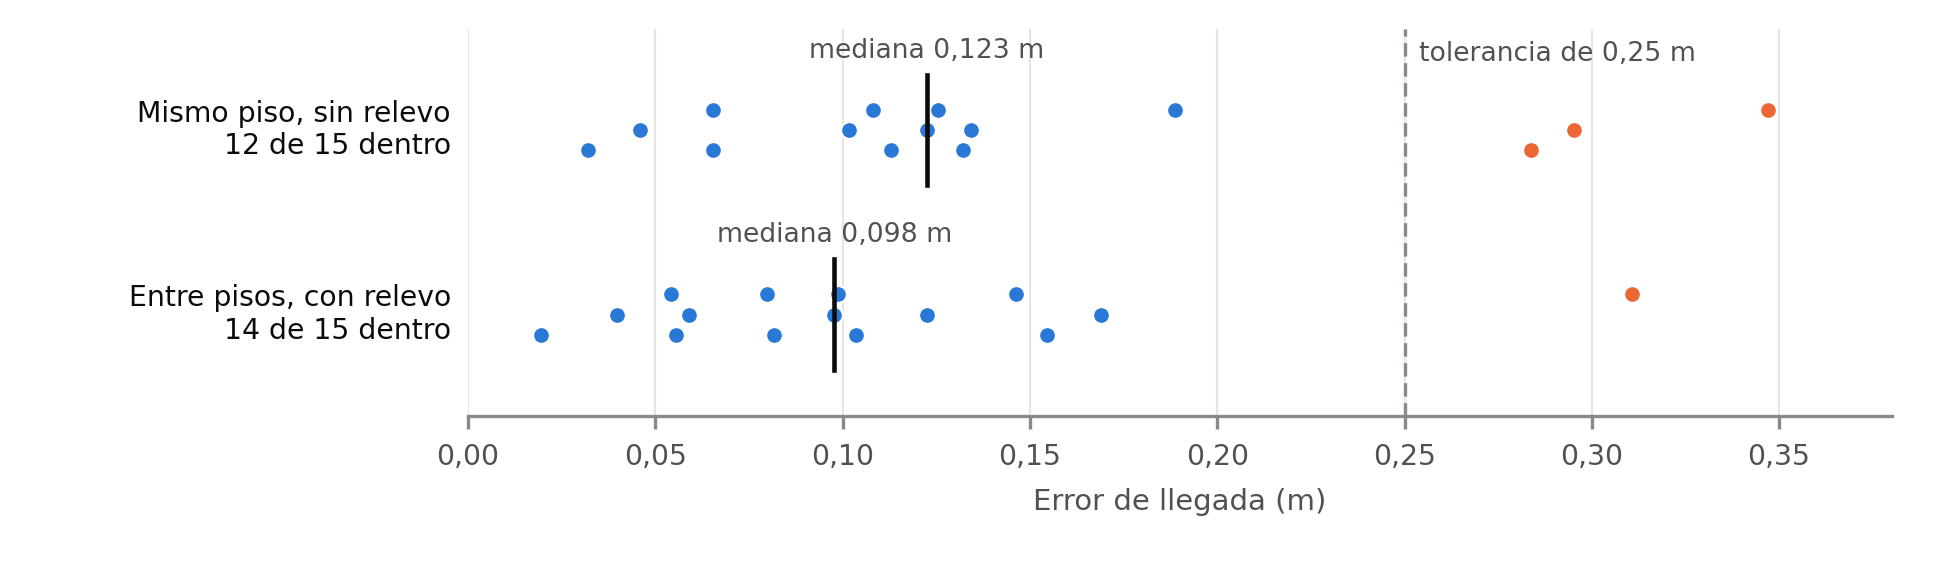
\includegraphics[width=0.8\textwidth]{imagenes/llegada_simulacion.png}
  \caption{Error de llegada de las treinta misiones en simulación, por grupo, con la tolerancia de 0,25~m (línea discontinua), las cuatro misiones fuera de ella (en naranja) y la mediana de cada fila (marca vertical).}
  \label{fig:llegada-sim}
\end{figure}

El tiempo de respuesta se presenta por escalones, sin media ni desviación, debido a que sus valores son múltiplos exactos de 100~ms, el paso con que avanza el reloj de la simulación: 0,1~s en diez misiones, 0,2~s en quince, 0,3~s en cuatro y 0,4~s en una. La cota, en cambio, sí se sostiene: el agente arranca en menos de medio segundo. El tiempo de asignación quedó por debajo de 100~ms en las treinta misiones, y en un banco de pruebas con el reloj del sistema tuvo una mediana entre 154 y 175~\textmu s y un máximo de 306~\textmu s.

% ---------------------------------------------------------------------
\section{Evaluación de la navegación con los agentes físicos}
\label{sec:res-hw}

La tabla~\ref{tab:odometria} reúne lo que midió la odometría en cada entorno, como fracción del avance real medido con flexómetro, frente al criterio de la prueba, un error de 10~\% o menos.

\begin{table}[H]
  \centering\footnotesize
  \caption{Fracción del avance real que registra la odometría, por entorno.}
  \label{tab:odometria}
  \begin{tabular}{@{}p{0.44\textwidth}ccl@{}}
    \toprule
    \textbf{Entorno} & \textbf{Recorrido} & \textbf{Registrado} & \textbf{Criterio} \\ \midrule
    Gregorio, pasillo simulado (46,9 m de extensión en su mapa) & largo & 37,9 \% & no cumple \\
    Gregorio, pasillos simulados de los pisos 2 y 3 & largo & 5,7 \% y 1,3 \% & no cumple \\
    Gregorio, hall del piso 3 & 6 m & 73 \% & no cumple \\
    Cuarto cerrado, desplazado a mano & 3 m & 96,3 -- 101,9 \% & cumple \\
    Catalayud, pasillo del piso 4 & 6,68 m & 95,4 \% & cumple \\
    Catalayud, pasillo del piso 4 & 14,57 m & 103,3 \% & cumple \\
    Catalayud, piso 4, con la unidad inercial & 8,08 m & 101,9 \% & cumple \\
    Catalayud, piso 4, con la unidad inercial & 2,82 m & 104,9 \% & cumple \\ \bottomrule
  \end{tabular}
\end{table}

El estimador es el mismo en todas las filas: lo que cambió fue el entorno. En un pasillo con hornacinas, casilleros y quiebres, la odometría queda dentro del $\pm$5~\% sin cambiar un parámetro. Las dos últimas filas ya incluyen la unidad inercial; el segundo de esos tramos mide 2,82~m, por debajo de los 5~m que pide el criterio, y se incluye como dato de la misma cadena.

La prueba de navegación de un agente pide un recorrido de punto a punto con Nav2 y la llegada verificada con flexómetro, a 0,5~m o menos del destino. En la primera sesión en el piso 4 del edificio Catalayud, el 2 de octubre, las dos llegadas medidas quedaron a 0,57 y 0,62~m, cortas, debido a que Nav2 daba entonces la meta por alcanzada a 1,0~m. El 7 de octubre, con la unidad inercial integrada y ese margen en 0,5~m, uno de los agentes recorrió en ese piso tres tramos encadenados, sin que nadie lo tocara entre uno y otro, y después regresó a la salida (tabla~\ref{tab:g3} y figura~\ref{fig:cadena}). Las llegadas medidas quedaron dentro de la tolerancia y la prueba se superó; al terminar cada tramo, la localización quedó a 0,10~m o menos de la medida en el sentido del avance y a 5~cm o menos de lado. La llegada al Salón 403 se estimó con el error de los otros dos tramos. El 8 de octubre, el otro agente recorrió el piso 3 en cinco tramos encadenados, con dos medias vueltas entre ellos, y los cinco terminaron con éxito y sin recuperaciones. Al forzar a la localización a recalcular su pose al final de cada tramo, esta se desplazó entre 0,61 y 0,86~m, debido a que la pose que publica al detenerse el agente va atrasada.

\begin{table}[H]
  \centering\footnotesize
  \caption{Cadena de tres tramos en el piso 4 del edificio Catalayud y regreso a la salida: llegada de cada tramo.}
  \label{tab:g3}
  \begin{tabular}{@{}llcccl@{}}
    \toprule
    \textbf{Tramo} & \textbf{Destino} & \textbf{Tiempo} & \textbf{Recuperaciones} & \textbf{A la meta} & \textbf{Medida} \\ \midrule
    1 & Salón 403 & 13,5 s & 1 & 0,26 m & estimada \\
    2 & Salón 402 & 27,8 s & 1 & 0,45 m & flexómetro \\
    3 & Salón 401 & 5,2 s & 0 & 0,06 m & flexómetro \\
    Regreso & Salida & 62,8 s & 6 & 0,34 m & flexómetro \\ \bottomrule
  \end{tabular}
\end{table}

\begin{figure}[H]
  \centering
  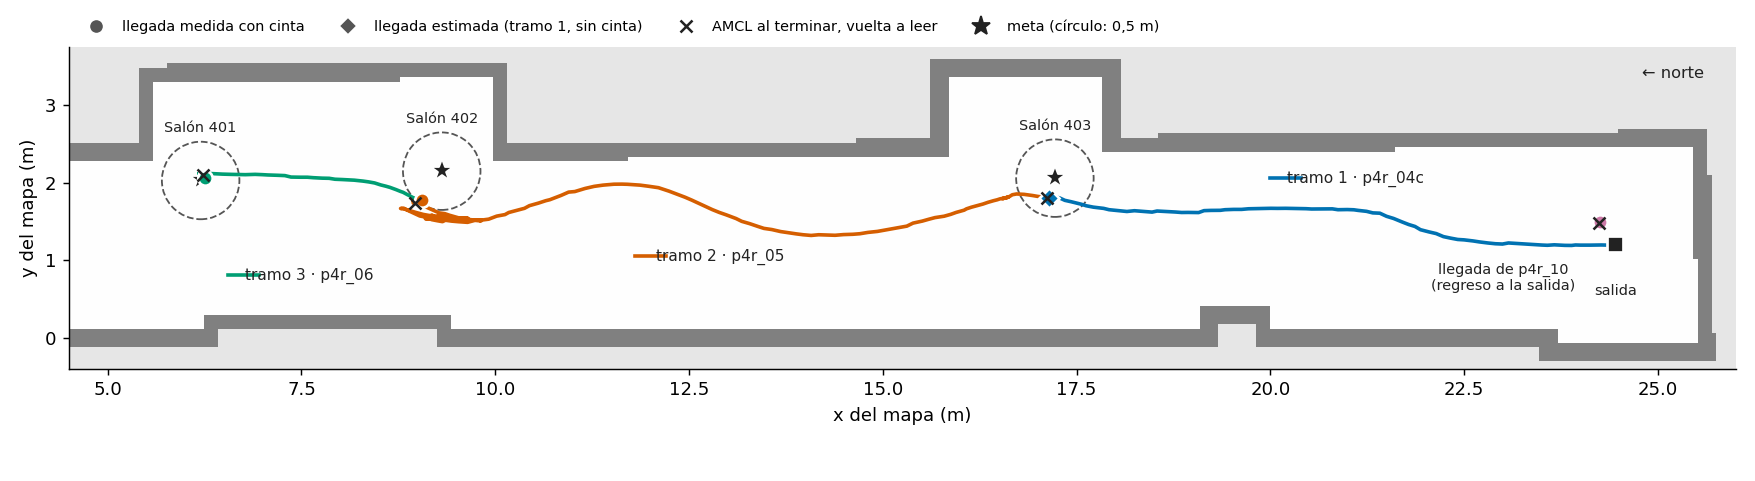
\includegraphics[width=0.78\textwidth]{imagenes/cadena_piso4.png}
  \caption{Cadena de tres tramos en el piso 4 del edificio Catalayud y regreso a la salida: recorrido según la localización, llegadas medidas con flexómetro y llegada estimada al Salón 403.}
  \label{fig:cadena}
\end{figure}

% ---------------------------------------------------------------------
\section{Evaluación del sistema completo con los agentes físicos}
\label{sec:res-completo}

El 16 de octubre, el sistema completo funcionó con los dos agentes físicos en los pisos 3 y 4 del edificio Catalayud (anexo A, video 7). Cada misión se pidió desde la página web en un teléfono, y los autores hicieron de usuario: acompañaron a los agentes y confirmaron el cambio de piso. Los agentes no se reubicaron entre misiones, y cuando el destino quedaba detrás del agente, el coordinador pidió la media vuelta en varios tiempos. La llegada se verificó con la localización de cada agente, que la prueba de navegación ya había comprobado con medidas directas (tabla~\ref{tab:g3}).

La primera prueba fue una misión del Salón 302 al Salón 402, que se completó en 132,5~s, con un relevo y con la llegada a 0,444~m del destino; entre la llegada del primer agente a la escalera y el arranque del segundo pasaron 61,1~s. Esa sesión sirvió de ensayo del montaje y sus misiones no forman parte de la campaña: de las doce grabadas, siete se completaron y cinco terminaron fallidas; en cuatro, el coordinador rechazó una llegada con el agente a entre 0,51 y 0,78~m del punto, y en la otra Nav2 abortó la navegación.

\subsection{La campaña con las misiones sorteadas}

De las diez misiones sorteadas, las nueve que llegaron a ejecutarse se completaron, todas con relevo (tabla~\ref{tab:campana-vehiculos}). Con nueve éxitos en nueve misiones, el intervalo de Wilson al 95~\% va del 70,1 al 100~\%, lo que permite afirmar que la tasa de éxito con los agentes físicos supera el 70~\%, la misma cota de la campaña en simulación. Con la expresión de la norma ASTM F3244-21, nueve repeticiones sin fallo demuestran una fiabilidad mínima de 0,81 con un 85~\% de confianza.

\begin{table}[H]
  \centering\footnotesize
  \caption{Las nueve misiones sorteadas de la campaña con los agentes físicos, todas completadas con un relevo.}
  \label{tab:campana-vehiculos}
  \begin{tabular}{@{}cllccc@{}}
    \toprule
    \textbf{N.\textsuperscript{o}} & \textbf{Origen} & \textbf{Destino} & \textbf{Tiempo total} & \textbf{Respuesta} & \textbf{Llegada} \\ \midrule
    1 & Ascensor, piso 3 & Salón 403 & 52,3 s & 0,51 s & 0,435 m \\
    2 & Salón 302 & Salón 401 & 90,1 s & 0,27 s & 0,202 m \\
    3 & Salón 401 & Salón 302 & 87,6 s & 3,90 s & 0,143 m \\
    4 & Salón 403 & Salón 303 & 78,9 s & 1,25 s & 0,420 m \\
    5 & Salón 402 & Salón 301 & 105,4 s & 0,66 s & 0,285 m \\
    6 & Salón 301 & Salón 401 & 89,8 s & 2,97 s & 0,226 m \\
    7 & Ascensor, piso 4 & Salón 301 & 81,7 s & 0,87 s & 0,234 m \\
    8 & Salón 302 & Salón 403 & 81,8 s & 0,95 s & 0,214 m \\
    9 & Salón 303 & Salón 402 & 92,6 s & 0,63 s & 0,299 m \\ \midrule
    \multicolumn{3}{@{}l}{Mediana} & 87,6 s & 0,87 s & 0,234 m \\ \bottomrule
  \end{tabular}
\end{table}

La mediana del error de llegada fue de 0,234~m, con valores de 0,143 a 0,435~m, y la del tiempo total, de 87,6~s, entre 52,3 y 105,4~s. En cuanto al tiempo de respuesta, su mediana fue de 0,87~s y quedó por debajo de 1,3~s en siete de las nueve misiones; los dos valores más altos, 3,90 y 2,97~s, son de misiones en que el agente ya estaba en el punto de origen. Medido con el reloj del portátil, el tiempo de asignación fue de 0,3~ms en las nueve misiones. En total, los agentes hicieron 24 medias vueltas, de entre 160 y 171$^\circ$, en uno a cuatro tiempos cada una.

La figura~\ref{fig:campana-vehiculos} descompone el tiempo de cada misión en sus etapas. Ir a recoger al usuario tomó entre 2,2 y 30,6~s, según dónde había terminado la misión anterior, mientras que el guiado en el piso de origen tuvo una mediana de 24,2~s, y el guiado en el piso de destino, de 24,8~s.

\begin{figure}[H]
  \centering
  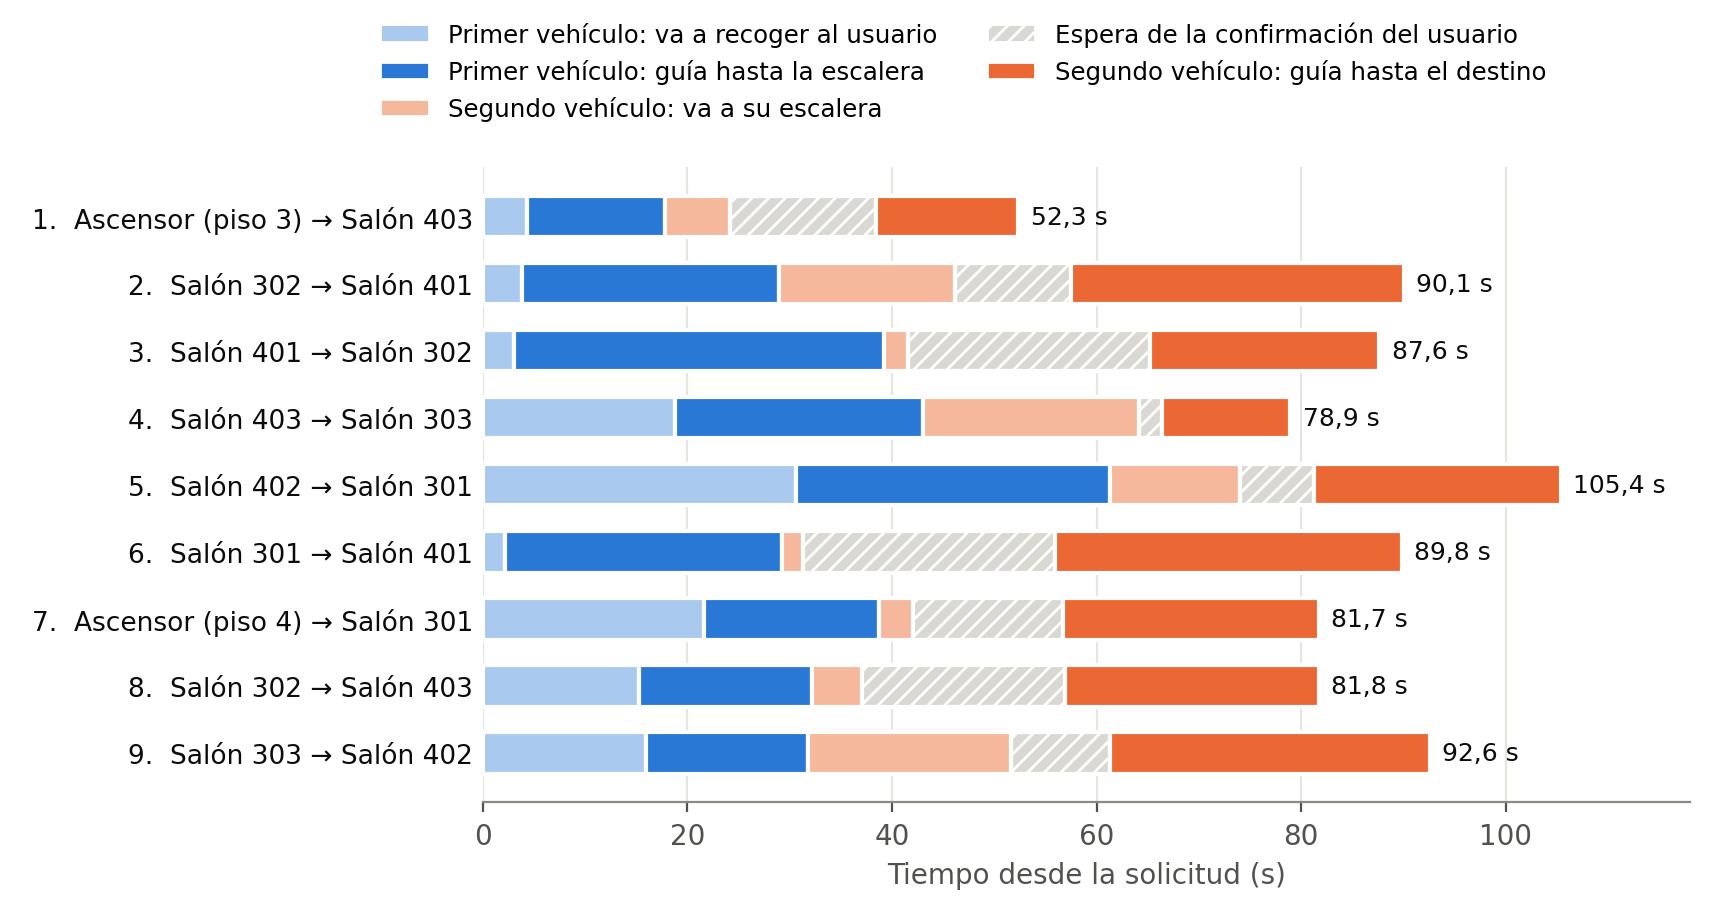
\includegraphics[width=0.64\textwidth]{imagenes/campana_vehiculos_etapas.png}
  \caption{Duración de cada etapa en las nueve misiones de la campaña con los agentes físicos, con la espera de la confirmación de piso en rayado.}
  \label{fig:campana-vehiculos}
\end{figure}

\subsection{El relevo entre los dos agentes}

El intervalo del relevo, desde que el primer agente llega a su escalera hasta el primer movimiento del segundo, tuvo una mediana de 1,22~s, cifra que junta dos situaciones. En cinco misiones el segundo agente tuvo que desplazarse hasta su escalera y arrancó en menos de 1,3~s. En las otras cuatro ya estaba en ella, y el intervalo, de 12,9 a 27,5~s, mide sobre todo cuánto tardó el usuario en confirmar.

El tiempo entre la llegada a la escalera del piso de origen y el arranque del guiado en el piso de destino, durante el cual el usuario cambia de piso y confirma en la página, tuvo una mediana de 24,8~s y fue de 18,0 a 29,5~s. La confirmación tomó entre 2,3 y 24,7~s, y el aviso de los 60~s no llegó a mostrarse en ninguna misión.

\subsection{Criterio de conteo e incidencias}

En la tasa de éxito cada misión cuenta una sola vez, con el intento que se completó, mientras que el protocolo cuenta como fallo toda ejecución fallida, por lo que se declaran los intentos que la tasa deja fuera. Las misiones 1 y 2 se completaron al segundo intento: en el primero de la misión 1, el coordinador rechazó la llegada al ascensor con el agente a 0,526~m del punto, y en el de la misión 2 no tenía la pose del agente para verificar la llegada.

Antes de esos intentos, la navegación de los dos agentes dejó de responder, y ocho intentos de la misión 1 terminaron rechazados o abortados. La detención ocurrió después de que el portátil se apagara por falta de batería, con los agentes ya con horas encendidos. Se reiniciaron las cadenas de navegación con la pose de salida, y después las nueve misiones se ejecutaron sin tocar los agentes. La misión 10 empezó y no terminó, pues el portátil volvió a apagarse por falta de batería poco después de pedirla. Antes se había pedido por error el ascensor del piso 4 como destino, debido a que los ascensores de los dos pisos aparecían en la página con el mismo nombre; ese intento no es una misión del sorteo y no se cuenta.

% ---------------------------------------------------------------------
\section{Limitaciones de la medición}
\label{sec:limitaciones}

La continuidad del servicio es la variable de respuesta principal del cuarto objetivo, y su criterio binario se cumplió en las treinta misiones. Ese resultado no es evidencia: el criterio exige que, dentro de la ventana de la misión, el coordinador nunca esté inactivo ni tenga el agente sin asignar, y los dos únicos puntos del código que producen esos valores ocurren antes de que la ventana se abra. La continuidad se declaró como un invariante estructural del diseño, y la afirmación se apoyó en una magnitud que sí varía, el intervalo del relevo, que en las quince misiones entre pisos tuvo una mediana de 0,1~s y un máximo de 0,2~s, es decir, uno o dos pasos del reloj de la simulación.

En el mapa de la campaña en simulación, el umbral con que se cargan las celdas libres era 0,25, y las celdas desconocidas, que el formato guarda con una ocupación de 0,196, quedaban por debajo de él: 10\,908 celdas que el modelo no describía, el 14,5~\% del mapa, se leyeron como espacio libre. El defecto no cambia el veredicto de la campaña, puesto que los cuatro fallos fueron de precisión de llegada y el pasillo por el que se navegó es libre. Queda sin verificar que ninguna trayectoria cruzara una de esas celdas. El umbral se corrigió a 0,10 el 25 de septiembre, tras la campaña.
